%===================================================================================
\section{Status of Higgs coupling fits}
%===================================================================================

We begin by showing in Fig.~\ref{fig:rcfit-ATLAS-CMS} contours of constant confidence level ...

\begin{figure}[h!]\centering
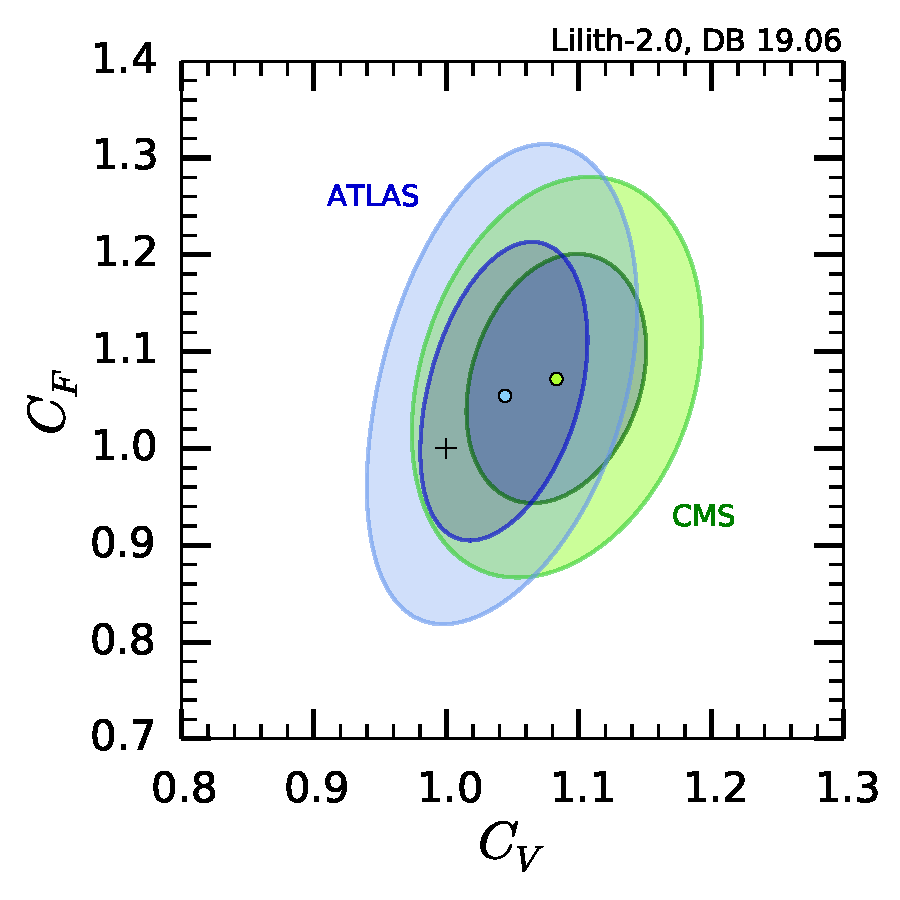
\includegraphics[width=0.45\textwidth]{fits/CVCF_2d_ATLAS_CMS.pdf}%
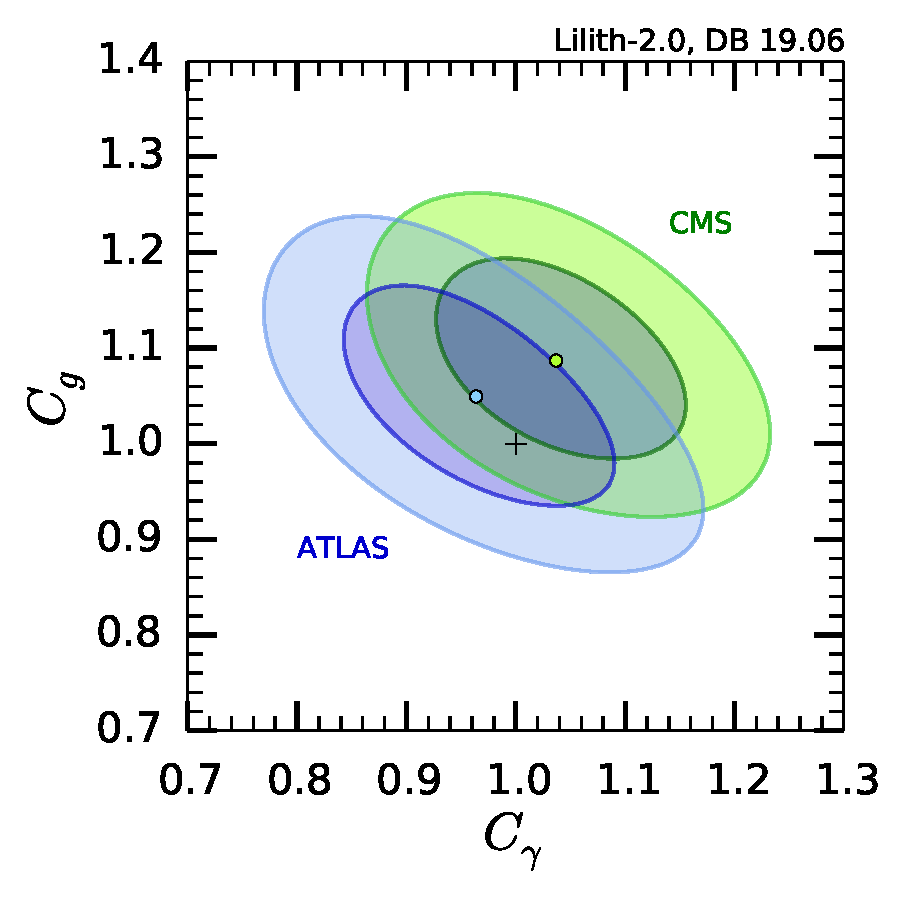
\includegraphics[width=0.45\textwidth]{fits/CgCGa_2d_ATLAS_CMS.pdf}%
\vspace*{-2mm}
\caption{Fit of $C_F$ vs.\ $C_V$ (left) and $C_g$ vs.\ $C_\gamma$ (right) using the Run~2 dataset of the 
current database version, DB~19.06. The 68\% and 95\% CL regions for the combined ATLAS results 
are shown in blue, those for CMS in green.}
\label{fig:rcfit-ATLAS-CMS}
\end{figure}

\begin{figure}[h!]\centering
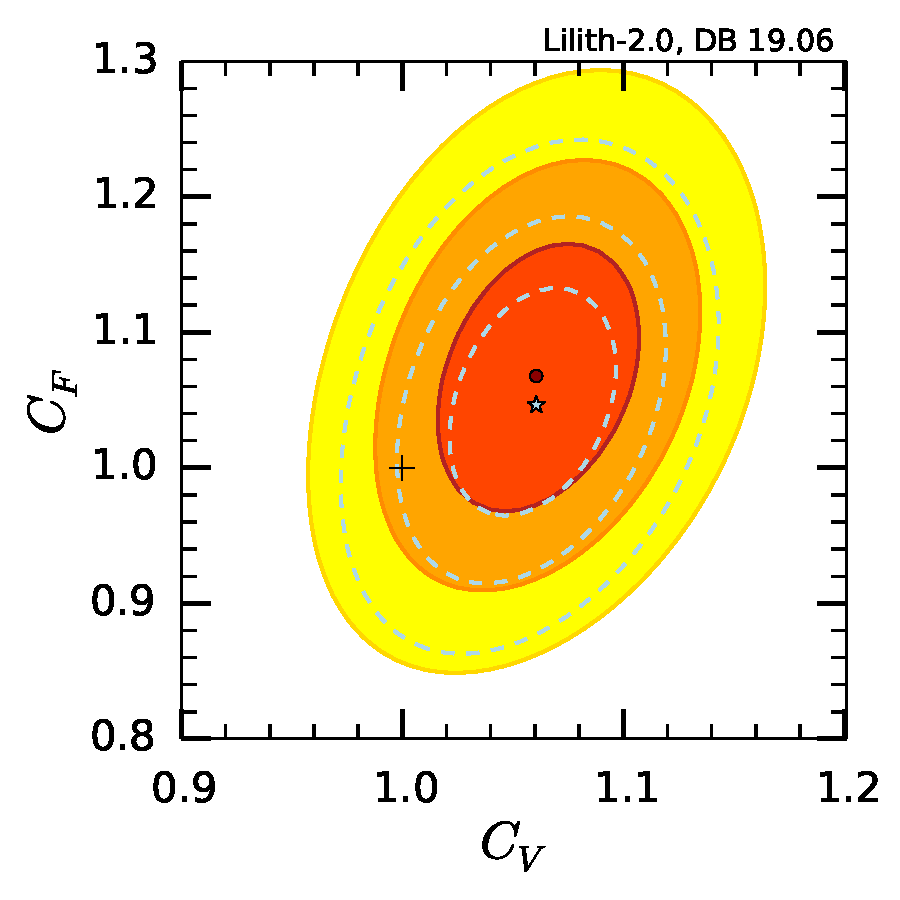
\includegraphics[width=0.45\textwidth]{fits/CVCF_2d_comb.pdf}%
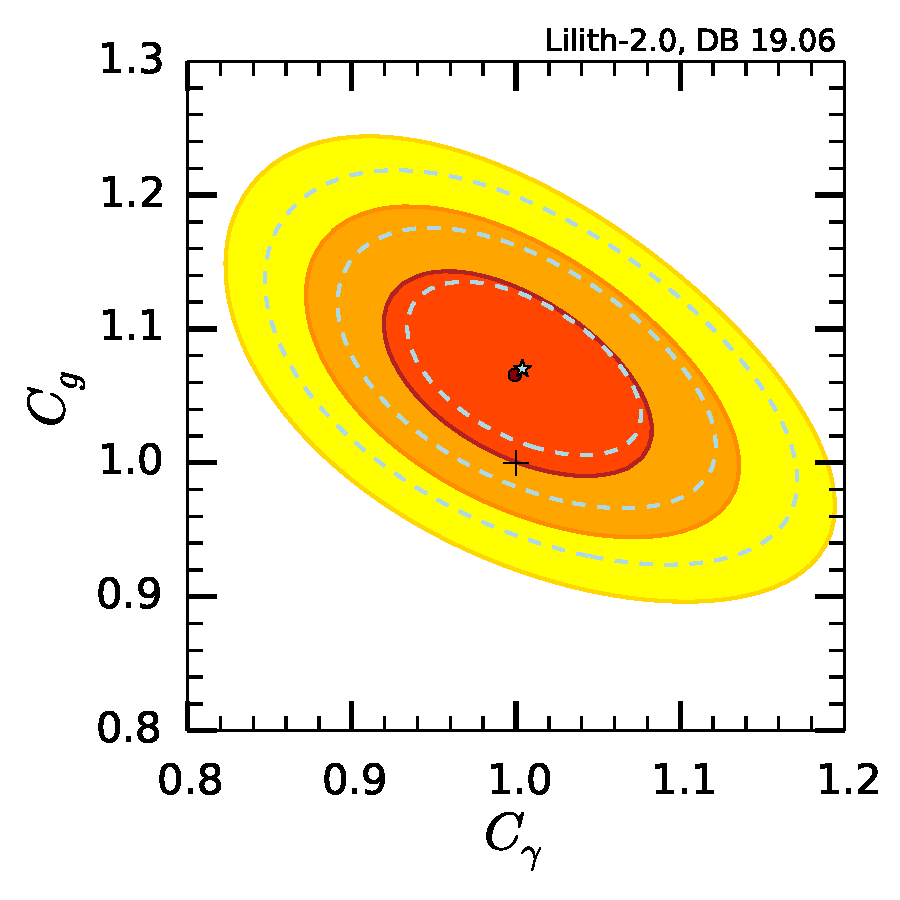
\includegraphics[width=0.45\textwidth]{fits/CgCGa_2d_comb.pdf}%
\vspace*{-2mm}
\caption{Fit of $C_F$ vs.\ $C_V$ (left) and $C_g$ vs.\ $C_\gamma$ (right) from a combination of the ATLAS and CMS 
Run~2 results in DB~19.06; the 68\%, 95\% and 99.7\% CL regions are shown as red, orange and yellow areas, respectively. 
In addition, the light blue dashed contours indicate the 68\%, 95\% and 99.7\% CL regions when combining the Run~2 and Run~1 data.}
\label{fig:rcfit-comb}
\end{figure}
